% ChronoJEPA working paper.
% Self-contained: compiles with a standard TeX install via `pdflatex paper && bibtex paper && pdflatex paper && pdflatex paper`.
% To retarget to a venue: replace \documentclass{article} and the geometry line with the venue
% style, e.g. \documentclass{article}\usepackage{neurips_2024} (place neurips_2024.sty alongside),
% or \documentclass{article}\usepackage{iclr2025_conference,times}. The body and bibliography are
% venue-agnostic.
\documentclass[11pt]{article}
\usepackage[margin=1in]{geometry}
\usepackage{amsmath,amssymb}
\usepackage{booktabs}
\usepackage{graphicx}
\usepackage{array}
\usepackage{microtype}
\usepackage[numbers]{natbib}
\usepackage[hidelinks]{hyperref}
\graphicspath{{../figures/}{figures/}}

\title{When Does the Time-Axis Collapse Matter? Disentangling Collapse,
Positional Structure, and Representation Richness in SIGReg-Regularised
Time-Series Representations}
\author{Rishabh Patil \\ University of St Andrews}
\date{}

\begin{document}
\maketitle

\begin{abstract}
LeJEPA \citep{lejepa2025} replaces the heuristic machinery of self-supervised learning with a
single isotropic-Gaussian regulariser, SIGReg, applied with no stop-gradient, no teacher, and no
schedulers. Carrying SIGReg to sequence models raises a documented hazard: a naive pooled
application can drive each sequence to a constant vector along time, a time-axis collapse that the
objective does not penalise. We build a self-supervised time-series library around this question
and compare three placements of SIGReg relative to the time axis: \emph{pooled} (the baseline),
\emph{dual} (SIGReg within each sequence across time plus across the batch), and \emph{structured}
(a joint variant). We confirm that the collapse is real and that the placement controls it: dual
robustly raises across-time variance by roughly an order of magnitude relative to pooled.

Our central finding is negative and clarifying. Through a factorial that crosses encoder
architecture with placement and probe feature, we show that the across-time variance collapse does
not measure downstream order availability, and in our experiments it is anticorrelated with it. The
determinant of whether a representation retains temporal order is the encoder's positional
structure, an axis orthogonal to the placement that controls the collapse. A position-free encoder
yields a permutation-invariant pooled feature whose order recovery is exactly chance on a
content-matched probe on two datasets, while a positional transformer, even when maximally
collapsed, recovers order at $0.97$ to $1.00$. The result holds across three architectures and two
datasets. The dual placement is nonetheless useful where the task needs the richer representation
it produces: on UCI HAR activity recognition dual beats pooled by $8$ to $11$ accuracy points under
both linear and nonlinear probes, and on forecasting, with eight seeds and paired significance
tests, dual is significantly better on ETTh2 and ETTm1, significantly worse on PEMS, and not
different on ETTh1. We propose a two-axis account: preventing the collapse does not change order
availability (set by positional structure) but increases representation richness (higher effective
rank), which helps downstream tasks whose targets are structured rather than near-constant.
\end{abstract}

\section{Introduction}

Self-supervised representation learning has converged on a small set of recurring devices:
asymmetric encoders, stop-gradients, momentum teachers \citep{byol2020}, predictor heads
\citep{simsiam2021}, and variance or covariance penalties \citep{vicreg2022,barlowtwins2021}.
LeJEPA \citep{lejepa2025} argues much of this can be replaced by a single objective. SIGReg
regularises a batch of embeddings toward an isotropic Gaussian by lifting a univariate normality
test to many dimensions through random projections, paired with a plain invariance term across two
augmented views, with no stop-gradient, teacher, EMA, or scheduler. It is natural to ask whether
this transfers to time series, where the dominant encoders are patching transformers
\citep{patchtst2023} and temporal convolutions \citep{tcn2018}.

A specific hazard motivates this work. When SIGReg is applied to one pooled embedding per sequence,
nothing prevents each sequence from converging to a constant vector along time while the pooled
batch still looks Gaussian: a time-axis analogue of dimensional collapse \citep{dimcollapse2022}.
The obvious fix applies SIGReg within each sequence across time, the dual placement, against the
pooled baseline. We set out to measure which placement best prevents the collapse and yields the
best downstream representations. We confirm the first half quickly. The second half is where the
work becomes interesting: a sequence of falsifiable predictions about downstream benefit are
refuted by the data, and the refutations compose into a cleaner account than the one we began with.

\paragraph{Contributions.}
(1) A heuristics-free SIGReg time-series library with three placements behind a common interface,
univariate tests ground-truthed against scipy, and reproducible diagnostics and probes.
(2) The finding that the across-time variance collapse diagnostic does not track downstream order
availability and is anticorrelated with it, established by a factorial over three architectures,
two placements, and two probe features, on two datasets, with a permutation-invariance proof and an
exact chance anchor.
(3) The identification of positional encoding as the determinant of order availability, via an
ablation and a temporal-convolution control that place the effect on a graded architectural axis.
(4) A two-axis account separating order availability (architecture) from representation richness
(placement), supported by a real labeled task (UCI HAR) and multi-dataset forecasting with paired
significance tests, including a corrected overclaim where a three-seed advantage did not survive
eight seeds.
(5) A negative result on label-free model selection by SIGReg loss for time-series forecasting.

\section{Method}

\paragraph{SIGReg.} For embeddings $Z \in \mathbb{R}^{N\times D}$, SIGReg samples $K$ unit
directions, forms projections $P = ZW \in \mathbb{R}^{N\times K}$, and for each slice computes the
Epps-Pulley statistic \citep{eppspulley1983} of the projected values against the standard normal
characteristic function, integrating $\big(C(t) - e^{-t^2/2}\big)^2 + S(t)^2$ over $t\in[0,t_{\max}]$
where $C,S$ are the empirical cosine and sine transforms. The integrand is even in $t$, so we
integrate over the half line and double; the statistic is validated against scipy quadrature, is
differentiable, and agrees on CPU and Apple MPS. We compare to the standard normal directly
(without per-slice standardisation) because the regulariser targets $N(0,I)$ and must see location
and scale deviations.

\paragraph{Placements.} An encoder maps a window to tokens $T\in\mathbb{R}^{B\times L\times D}$ and
a pooled embedding (mean over time). \emph{Pooled} applies SIGReg to the pooled embedding (the
collapse source). \emph{Dual} applies SIGReg within each sequence across time (the $L$ tokens as
$N=L$ samples) plus across the batch; the within-sequence term is large exactly when a sequence
collapses. \emph{Structured} applies SIGReg jointly to all per-timestep embeddings $(B L, D)$. The
loss is $\lambda\,\mathrm{sigreg} + (1-\lambda)\,\mathrm{invariance}$ with a single knob.

\paragraph{Encoders.} Three encoders share the contract $(B,C,T)\to(\text{tokens }(B,L,D),
\text{pooled }(B,D))$: PatchTST \citep{patchtst2023} (positional transformer), a TCN
\citep{tcn2018} (positional via convolution), and a position-free bag-of-patches encoder that
embeds non-overlapping patches independently with a shared MLP and no positional encoding or
cross-patch interaction. We prove and unit-test that the bag-of-patches encoder is
permutation-equivariant over patches, so its pooled feature is permutation-invariant; we likewise
unit-test that removing positional encoding makes the transformer over patches
permutation-equivariant.

\paragraph{Diagnostics and probes.} Across-time variance is the mean variance of the token
embedding along time (near zero under collapse); effective rank \citep{effrank2007} is
$\exp(\mathrm{entropy}(\text{normalised singular values}))$. All evaluation uses a frozen encoder
and a linear or nonlinear MLP probe on either the pooled feature or the flattened token sequence.
To isolate order we build two labels from the windows: \emph{trend} (is the second-half mean above
the first-half mean) and \emph{halfswap} (a window against the same window with its two halves
swapped, content-matched, varying only position). Forecasting probes a linear head on frozen
features against the next-horizon trajectory. Splits are time-ordered and scalers fit on train
only.

\section{Experimental setup}

Datasets: PEMS08 traffic flow \citep{astgcn2019} (170 channels, five-minute), the ETT family
\citep{informer2021} ETTh1, ETTh2 (hourly) and ETTm1 (fifteen-minute, seven channels), and UCI HAR
\citep{ucihar2013} (nine inertial channels, $128$-step windows, six activities). Unless noted,
encoders use $d_{\text{model}}\in\{32,64\}$ as stated, two transformer layers, four heads, patch
length $16$, stride $8$, $32$ slices, $\lambda=0.5$, two-view augmentation, $500$ steps, AdamW with
a cosine schedule. We report mean and standard deviation over seeds, and for forecasting a paired
$t$-test with a $95\%$ bootstrap CI on the seed-aligned dual-minus-pooled difference.

\section{Results}

\subsection{The collapse is real and placement-controlled, and benign for PEMS forecasting}

On PEMS08 over five seeds, pooled across-time variance is $0.064\pm0.007$ against dual
$0.607\pm0.008$ (non-overlapping), confirming the placement controls the collapse. We expected dual
to forecast better; it does not on PEMS. With a trajectory probe pooled is reliably slightly better,
and a horizon sweep refutes the near-persistence explanation: pooled stays $0.005$ to $0.007$ MAE
better at every horizon from $3$ to $48$. A Mahalanobis anomaly comparison saturates for both
placements (AUROC near $1.0$), because even a collapsed encoder remains content-sensitive.

\subsection{The factorial: across-time variance does not track order}

Table~\ref{tab:factorial} crosses architecture with placement and reports collapse diagnostics and
halfswap and trend accuracy from token and pooled features on PEMS08 (five seeds).

\begin{table}[t]
\centering\small
\caption{Architecture $\times$ placement factorial on PEMS08 (five seeds). The position-free
bag-of-patches pooled feature recovers a content-matched half-swap at exactly chance ($0.500$),
while the positional transformer recovers it at $0.97$ even at its lowest variance. Across-time
variance is anticorrelated with order.}
\label{tab:factorial}
\begin{tabular}{l ccccc}
\toprule
arch $\mid$ placement & across-time var & eff.\ rank & halfswap (tok) & halfswap (pool) & trend (pool) \\
\midrule
positional $\mid$ pooled   & $0.111\pm0.015$ & $6.47$  & $1.000$ & $0.977$ & $0.953$ \\
positional $\mid$ dual     & $0.612\pm0.011$ & $8.31$  & $1.000$ & $0.973$ & $0.964$ \\
tcn $\mid$ pooled          & $1.467\pm0.217$ & $8.23$  & $0.931$ & $0.522$ & $0.862$ \\
tcn $\mid$ dual            & $5.247\pm1.633$ & $6.25$  & $0.982$ & $0.651$ & $0.888$ \\
bagofpatches $\mid$ pooled & $1.661\pm0.131$ & $1.45$  & $0.502$ & $\mathbf{0.500}$ & $0.887$ \\
bagofpatches $\mid$ dual   & $1.697\pm0.093$ & $1.62$  & $0.489$ & $\mathbf{0.500}$ & $0.897$ \\
\bottomrule
\end{tabular}
\end{table}

The lowest-variance configuration (positional, pooled) recovers order best, and the high-variance
bag-of-patches recovers none; the TCN is intermediate, retaining order in token features and
partially in pooled features. Order availability is graded by how globally the architecture mixes
position. Effective rank also dissociates from variance (bag-of-patches: high variance, lowest
rank). Figure~\ref{fig:halfswap} shows the half-swap result.

\begin{figure}[t]
\centering

\includegraphics[width=0.85\linewidth]{halfswap.png}
\caption{Half-swap order recovery on PEMS08. The positional transformer recovers order from both
features in every placement; the position-free bag-of-patches encoder sits at the chance line
($0.5$) regardless of placement or feature. Order availability tracks architecture, not the
placement that controls collapse.}
\label{fig:halfswap}
\end{figure}

\paragraph{Ablation.} Probing the pooled time-mean feature (a simulated full collapse) still
recovers half-swap at $\sim0.98$ on PEMS, because positional encoding and attention write order into
token values before pooling. Removing positional encoding (the transformer then being
permutation-equivariant) drops pooled-feature half-swap from $\sim0.98$ toward $0.90$; the clean
chance result is the bag-of-patches encoder. Positional encoding, not the absence of collapse, is
what lets a collapsed representation keep order.

\subsection{External validity: ETT and multi-dataset forecasting}

The factorial replicates on ETTh1: the position-free pooled feature is again at exactly $0.500$ on
half-swap, and trend from the pooled feature separates the positional encoder ($0.72$ to $0.77$)
from the position-free one ($0.54$, chance). Table~\ref{tab:forecast} reports eight-seed forecasting
with paired significance.

\begin{table}[t]
\centering\small
\caption{Trajectory-forecasting MAE across four datasets, eight seeds, with a paired $t$-test and a
$95\%$ bootstrap CI on the dual-minus-pooled gap. The significance pass corrected an earlier
three-seed ETTh1 advantage that does not survive.}
\label{tab:forecast}
\begin{tabular}{l ccccl}
\toprule
dataset & pooled MAE & dual MAE & gap & $p$ & $95\%$ CI on gap \\
\midrule
PEMS08 & $0.4421$ & $0.4563$ & $+0.0142$ & $0.001$ & $[+0.009,+0.019]$ (pooled) \\
ETTh1  & $1.1833$ & $1.1614$ & $-0.0219$ & $0.52$  & $[-0.086,+0.033]$ (null) \\
ETTh2  & $0.8589$ & $0.7378$ & $-0.1211$ & $0.0004$& $[-0.156,-0.088]$ (dual) \\
ETTm1  & $0.6337$ & $0.5843$ & $-0.0494$ & $<10^{-4}$ & $[-0.056,-0.043]$ (dual) \\
\bottomrule
\end{tabular}
\end{table}

Dual is significantly better on ETTh2 and ETTm1, significantly worse on PEMS, and not different on
ETTh1. The forecasting benefit is capacity gated (vanishing at $d_{\text{model}}=32$) and largest at
short horizons, contrary to our prediction that it would grow with horizon; it is a richness effect,
not an order or horizon effect. Dual is also several times more stable across seeds.

\subsection{A real labeled task: HAR activity recognition}

Table~\ref{tab:har} reports the SSL pretrain-then-probe comparison on UCI HAR (five seeds), the
clearest case where preventing the collapse helps. Dual beats pooled by $8$ to $11$ accuracy points
on every probe, under both linear and nonlinear MLP readouts (so not a linear artifact) and from
both features, with non-overlapping bands; pooled is heavily collapsed (variance $0.019$) and
classifies poorly while dual is uncollapsed ($0.602$). Figure~\ref{fig:har}.

\begin{table}[t]
\centering\small
\caption{UCI HAR test accuracy, SSL pretrain then frozen probe (five seeds).}
\label{tab:har}
\begin{tabular}{l ccccc}
\toprule
placement & linear (pool) & MLP (pool) & linear (tok) & MLP (tok) & across-time var \\
\midrule
pooled & $0.576\pm0.008$ & $0.633\pm0.014$ & $0.636\pm0.009$ & $0.679\pm0.016$ & $0.019\pm0.003$ \\
dual   & $0.655\pm0.023$ & $0.718\pm0.021$ & $0.740\pm0.024$ & $0.788\pm0.023$ & $0.602\pm0.052$ \\
\bottomrule
\end{tabular}
\end{table}

\begin{figure}[t]
\centering
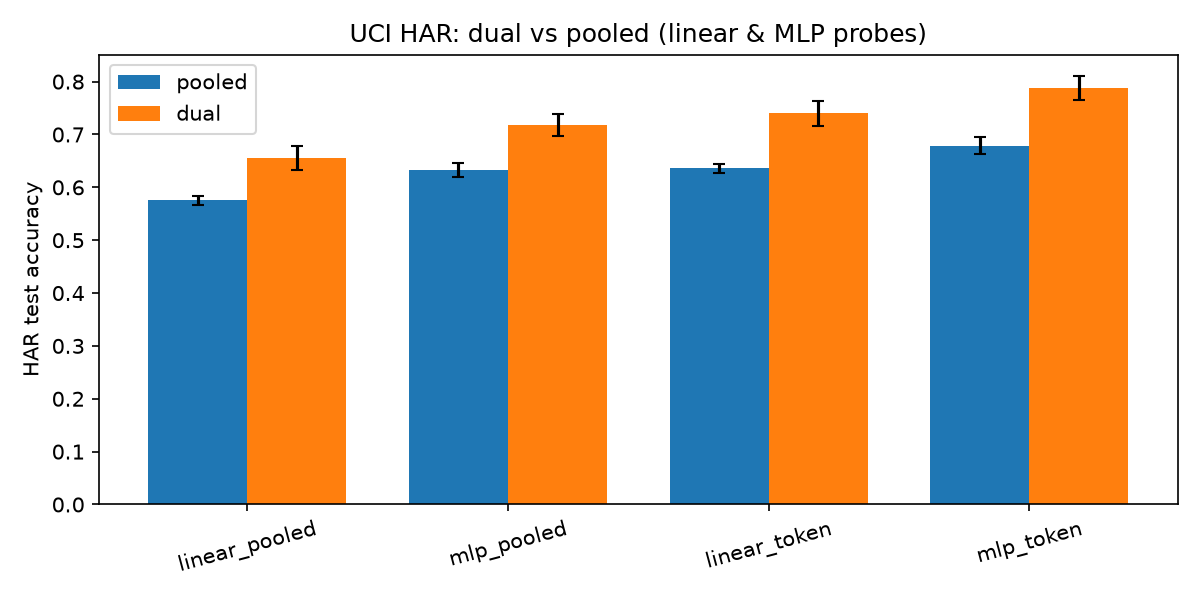
\includegraphics[width=0.8\linewidth]{har_classification.png}
\caption{UCI HAR: dual versus pooled under linear and MLP probes on pooled and token features. Dual
wins by $8$ to $11$ points on every probe, with non-overlapping error bars.}
\label{fig:har}
\end{figure}

Running the comparison across all three architectures (Table~\ref{tab:har_arch}, MLP on token
features, three seeds) ties dual's benefit causally to the collapse it prevents. The gain is largest
on the positional transformer, which collapses most under the pooled placement (across-time
variance $0.017$) and gains $7$ to $10$ points; moderate on the TCN; and negligible on the
position-free bag-of-patches, which barely collapses ($0.281$) and so leaves dual little to add.
Dual helps exactly where preventing the collapse has something to prevent.

\begin{table}[t]
\centering\small
\caption{HAR across architectures (three seeds, MLP probe on token features). The dual gain tracks
how much the pooled baseline collapses.}
\label{tab:har_arch}
\begin{tabular}{l ccc cc}
\toprule
architecture & pooled acc & dual acc & dual gain & pooled var & dual var \\
\midrule
positional   & $0.672\pm0.017$ & $0.773\pm0.019$ & $+0.101$ & $0.017$ & $0.578$ \\
tcn          & $0.826\pm0.015$ & $0.869\pm0.023$ & $+0.044$ & $1.772$ & $4.384$ \\
bagofpatches & $0.722\pm0.008$ & $0.733\pm0.009$ & $+0.011$ & $0.281$ & $0.353$ \\
\bottomrule
\end{tabular}
\end{table}

\subsection{Label-free model selection}

A $\lambda$ sweep shows across-time variance is set by placement, not $\lambda$, and that SIGReg is
in mild tension with forecasting (higher $\lambda$ raises effective rank but worsens dual's MAE). We
tested LeJEPA's label-free selection claim that final SIGReg loss tracks downstream performance: it
does not transfer here. The cross-configuration Spearman correlation is $0.552$ ($p=0.098$) and the
label-free pick disagrees with the label-based pick; moreover the correlation is confounded by the
two placements having different SIGReg loss scales (dual sums two terms), and within a placement the
relationship is flat or reversed.

\section{Discussion}

The results compose into a two-axis account. \emph{Order availability}, whether a readout can
recover temporal order, is governed by the encoder's positional structure and is essentially
untouched by the placement or the collapse: a positional transformer keeps order even when
collapsed, a position-free encoder loses it regardless, a convolution sits between. The collapse
diagnostic does not measure this axis and runs opposite to it. \emph{Representation richness},
proxied by effective rank, is increased by the dual placement, and whether it helps depends on
whether the task needs it: not on near-persistence forecasts (PEMS), yes on structured forecasts
(ETTh2, ETTm1) and a real order-dependent classification task (HAR). For SIGReg on time series this
reframes the practical guidance: the time-axis collapse is genuine and dual fixes it, but on the
positional encoders that dominate the field the collapse is not the right quantity to monitor, and
the dual placement should be motivated by the richness it adds rather than as a universal remedy.

\section{Limitations}

Forecasting uses a frozen-feature probe rather than the standard lookback-to-horizon protocol with a
tuned baseline such as DLinear \citep{dlinear2023}, so absolute errors are representation-quality
measurements, not state of the art. The five datasets span three domains and the ETT variants are
closely related. Training is fixed at $500$ steps and not shown converged. The richness-to-benefit
link is correlational through effective rank, not causally isolated. The synthetic order probes have
dataset-dependent confounds, which we document and mitigate with the exact chance anchor.

\section{Conclusion}

We extended SIGReg to time series, confirmed the time-axis collapse and that dual prevents it, and
showed through a factorial across three architectures and two datasets that the collapse diagnostic
does not measure downstream order availability and is anticorrelated with it, the true determinant
being positional encoding. We separated order availability (architecture) from representation
richness (placement) and showed, with significance tests and a real labeled task, that dual helps
where the task needs richness and not where it does not. Future work should run the factorial on
further real labeled datasets, anchor forecasting to standard baselines, and probe the
richness-to-benefit link causally.

\small
\bibliographystyle{plainnat}
\bibliography{references}

\end{document}
